\documentclass[12pt,a4paper]{article}

\usepackage[left=3cm,right=2cm,top=2.5cm,bottom=1.5cm,includeheadfoot]{geometry}

\usepackage[english, ngerman]{babel}
\usepackage{amsmath}
\usepackage{graphicx}
\usepackage{xcolor}
\usepackage{makeidx}

% Blindtext
\usepackage{blindtext}
\usepackage{lipsum}

% Umlaute
\usepackage[utf8]{inputenc}

% Verbesserte Schrift
\usepackage{microtype}

% Verlinkungen
\usepackage{hyperref}

% Bessere Tabellen
\usepackage{array}
%\usepackage[table]{xcolor}

% Abkürzungsverzeichnis
\usepackage[nolist, nohyperlinks]{acronym}

% Figure a b
\usepackage{subcaption}

% Entfernt alle Bilder
%\usepackage[nolists,nomarkers]{endfloat}
%\renewcommand{\processdelayedfloats}{}

% !TEX root = main.tex
\hypersetup{
	pdftitle={GraalVM-NativeImage},
	pdfsubject={GraalVM-NativeImage},
	pdfauthor={Erik Simonsen},
	pdfkeywords={Java, GraalVM, NativeImage, JVM, HotSpotVM},
	pdfstartpage={1},
	plainpages=false,
	hypertexnames=false
}

% !TEX root = main.tex
\usepackage{listings}
\usepackage{accsupp}
\usepackage[margin=12pt]{caption}

% LstListing Color
\definecolor{commentGreen}{rgb}{0,0.6,0}
\definecolor{numberGray}{rgb}{0.25,0.25,0.25}
\definecolor{stringMauve}{rgb}{0.08,0.52,0.1}
\definecolor{backgroundGray}{rgb}{0.98,0.98,0.98}

\lstset{ %
	abovecaptionskip=12pt,
	backgroundcolor=\color{backgroundGray},
	basewidth=0.5em,
	basicstyle=\small\ttfamily,
	breakatwhitespace=false,
	breaklines=true,
	captionpos=b,
	columns=flexible,
	commentstyle=\color{commentGreen},
	deletekeywords={...},
	escapeinside={(*@}{@*)},
	extendedchars=false,
	frame=lr,
	framesep=20pt,
	framerule=0pt,
	keepspaces=true,
	keywordstyle=\color{blue},
	language=Java,
	otherkeywords={my-component,export,@Component,@Directive,@Injectable,@Input,@Output,io-component,ee-node,ee-separator,ee-panel,ee-panel-header,ee-table},
	numbers=left,
	numbersep=5pt,
	numberstyle=\scriptsize\color{numberGray}\noncopynumber,
	rulecolor=\color{black},
	showspaces=false,
	showstringspaces=false,
	showtabs=false,
	stepnumber=1,
	stringstyle=\color{stringMauve},
	tabsize=4,
	title=\lstname,
	xleftmargin=0.5cm
}

\newcommand{\noncopynumber}[1]{
	\BeginAccSupp{method=escape,ActualText={}}
	#1
	\EndAccSupp{}
}

\renewcommand{\lstlistingname}{Codeausschnitt}
\usepackage{subcaption}
\usepackage{tikz-qtree}
\usetikzlibrary{positioning}

\definecolor{nodeRed}{HTML}{F44336}
\definecolor{nodeBlue}{HTML}{2196F3}
\definecolor{nodeYellow}{HTML}{FFEB3B}
\definecolor{nodeGreen}{HTML}{4CAF50}
\definecolor{nodeOrange}{HTML}{FF9800}
\definecolor{nodeGray}{HTML}{607D8B}

% Tikz Tree settings
\tikzset{every tree node/.style={draw, rectangle, minimum width=1.5em, minimum height=1.5em,line width=1pt}, level distance=1.3cm,sibling distance=0.5cm}
\tikzset{red/.style={draw, fill=nodeRed}}
\tikzset{blue/.style={draw, fill=nodeBlue}}
\tikzset{yellow/.style={draw, fill=nodeYellow}}
\tikzset{green/.style={draw, fill=nodeGreen}}
\tikzset{orange/.style={draw, fill=nodeOrange}}
\tikzset{gray/.style={draw, fill=nodeGray}}
\tikzset{white/.style={draw, fill=white}}
\tikzset{black/.style={draw, fill=black}}
% !TEX root = main.tex
\usepackage{ntheorem}
\usepackage{mdframed}

\theoremstyle{break}
\theoremheaderfont{\bfseries}
\newmdtheoremenv[
nobreak=true,
linecolor=red,
linewidth=2,
leftmargin=0,
rightmargin=0,
backgroundcolor=yellow,
innertopmargin=10pt,
ntheorem]{todo}{TODO}[section]

% für das Zitieren aus einer bib-Datei
%\usepackage[natbib=false,backend=biber,style=alphabetic]{biblatex}
%\usepackage[natbib=true,backend=bibtex,style=authoryear]{biblatex} So werden die Zitate und das Literaturverz. als Authorname + Erscheinungsjahr ausgegeben, allerdings werden keine eckigen Klammern darum gemacht, so das diese manuell gemacht werden müssen.
\usepackage[natbib=true,backend=bibtex,style=authoryear]{biblatex}
\def\BibTeX{{\rm B\kern-.05em{\sc i\kern-.025em b}\kern-.08em
    T\kern-.1667em\lower.7ex\hbox{E}\kern-.125emX}}
\usepackage{csquotes}
\bibliography{bib/bib.bib}
%\addbibresource{bib.bib}

% !TeX root = ba.tex
%\section{Abkürzungsverzeichnis}
\begin{acronym}
	\acro{fab}[FAB]{Floating Action Button}
\end{acronym}
\begin{document}

\pagestyle{empty}
\pagenumbering{roman}
% !TEX root = main.tex
\begin{minipage}{2.1cm}
	
\includegraphics[width=2cm]{resources/fh_logo_klein.jpg}
\end{minipage}
\begin{minipage}{10.0cm}
	Ostfalia - Hochschule für angewandte Wissenschaften\\
	Fakultät Informatik\\
	Studiengang Informatik
\end{minipage}

\vspace{35mm}

\begin{center}
	{\LARGE Seminar}\\[10mm]
\end{center}

\begin{center}
	\LARGE \textbf{GraalVM - NativeImage\\[28mm]}
\end{center}

\begin{table}[h]
	\centering
	\hspace{50mm}\begin{tabular}{lcll}
		eingereicht bei &  & Prof. Dr. B. Müller &          \\
		                &  &                     &          \\
		von             &  & Erik Simonsen     	 & 70455429 \\
		        
	\end{tabular}
\end{table}

\vspace{30mm}

\begin{table}[h]
	\begin{tabular}{lll}
		Wolfenbüttel, den \today\\
	\end{tabular}
\end{table}
\clearpage

% !TEX root = main.tex
\selectlanguage{ngerman}
\begin{abstract}
\normalsize
\noindent 
In den letzten Jahren ging der Trend in der Softwareentwicklung von Monolithen, die auf hohen Durchsatz ausgelegt waren, zu Microservices und zu Functions as a Service(FaaS), die 
auf kleine, in sich geschlossene Anwendungen ausgelegt sind, die oft gestartet werden. Dabei beeinflussen die Startzeit und der Speicherverbrauch direkt die erhobenen Kosten der Cloudanbieter.
Die Nutzung von Java spielte in diesen Bereichen bislang eher eine kleine Rolle, aufgrund der langsamen Startzeiten, benötigter Aufwärmzeiten und hohen Speicherverbrauchs der JVM. Ein Faktor dafür
 ist unter anderem die Funktionalität die Java zur Laufzeit bietet und es damit auch von anderen Sprachen abhebt, beispielsweise \textit{dynamic class loading}. Für Anwendungen, die solche Java-Features allerdings nicht nutzen, und zum Deployment der sog. 
Closed-World Annahme entsprechen, bietet die Native Image-Funktionalität von GraalVM schnelle Startzeiten und geringen Speicherverbrauch, und macht sie dadurch geeignet für genannte Anwendungsmodelle.
Dabei wird der Anwendungscode, dazugehörige Bibliotheken, die JVM und spezifische Virtual Machine-Komponenten in eine nativ ausführbare, in sich geschlossene Datei (\textit{native image bzw. executable}
durch ahead-of-time Kompiling kompiliert. Während des Build-Prozesses werden erhebliche Code-Optimierungen gemacht und der Heap des \textit{native image} wird bereits vorgefüllt. Dadurch wird eine, im Gegensatz zur Java Hotspot VM,
erhebliche Steigerung der Startzeit und des Speicherverbrauches erzielt.
\end{abstract}

\clearpage
\thispagestyle{empty}

\section*{Ehrenwörtliche Erklärung}

Hiermit erkläre ich ehrenwörtlich, dass ich das vorliegende Praxisprojekt selbstständig und ohne unerlaubte fremde Hilfe angefertigt habe, andere als die angegebenen Quellen nicht benutzt und die  benutzten Quellen wörtlich oder die inhaltlich entnommenen Stellen als solche kenntlich gemacht habe.
\vspace{4em}\\
Wolfenbüttel, den \today
% !TEX root = main.tex
\clearpage
\selectlanguage{ngerman}
\begingroup
\hypersetup{hidelinks}
\tableofcontents
\endgroup
\clearpage

\setcounter{page}{1}
\pagenumbering{arabic}
\pagestyle{headings}

% !TEX root = main.tex
\section{Einleitung}
\label{sec:einleitung}

\subsection{Motivation}
\label{subsec:motivation}
Softwareentwicklung hat sich in den letzten Jahren stark verändert, moderne Anwendungen setzen immer öfter auf Microservices und verschiedene Modelle des Cloud-Computings, wie
Serverless Computing. Statt große Anwendungsserver zu nutzen, werden dabei unabhängige Services deployed (Function as a Service, FaaS). Sobald die Workload steigt, also die Anzahl der Anfragen an den Service steigen,
werden von der jeweiligen Cloudplattform mehrere \textit{Worker} erstellt, welche die Anfragen bearbeiten. Bei der ersten Anfrage die ein neuer \textit{Worker} bearbeitet, muss zuerst die Laufzeitumgebung 
der jeweiligen Programmiersprache und die Konfiguration des Services initialisiert werden. Da solche Kaltstarts bei virtuellen Machinen häufig sehr langsam sind\footnote{Besonders bei Java VMs
 durch Ausführen von Class Loading, Profiling, dynamischer Kompilierung etc.} und Cloudanbieter nach Start- und Laufzeit einer Funktion abrechnen bietet sich die Nutzung von Java VMs nicht an.

\subsection{GraalVM}
\label{subsec:graalvm}

GraalVM ist ein Softwareprodukt von Oracle. Es wird als Ökosystem bezeichnet und die zentrale Komponente ist der \textit{GraalVM Compiler), ein in Java geschriebener JIT(Just-in-time)-Compiler für Java, der durch neue Codeanalyse- und 
 Optimierungsmethoden erhebliche Performancevorteile bietet.
Darüber hinaus bietet GraalVM die Möglichkeit der polyglotten Programmierung mithilfe des Truffle-Frameworks und der Ausführung von nativem Code auf der JVM, durch einen LLVM Bitcode Interpreter.
Zudem bietet GraalVM die \textit{Native Image} Funktionalität, die im weiteren Verlauf dieser Arbeit thematisiert wird. \textit{Native Image} ermöglicht das ahead-of-time kompilieren von Java-Anwendungen in nativ ausführbare Dateien (executables).
Die Grundlage von GraalVM bietet das OpenJDK\parencite{GraalComponents}.\newline

 Darin enthalten ist, neben Komponenten & Werkzeugen für die Entwicklung, auch die Java-Laufzeitumgebung (Java Runtime Environment, JRE), welche die HotSpot JVM enthält.
Die Hotspot JVM enthält zwei JIT-Compiler:  C1, einen schnellen und nur leicht optimierenden Compiler, ursprünglich gedacht für Desktopanwendungen, und C2, einen aggressiv optimierenden Compiler für 
Serveranwendungen, bei denen es auf höchsten Durchsatz ankommt.
Über das JMVCI (Java Virtual Machine Compiler Interface, \parencite{OpenJDK243}) wird der GraalVM-Compiler in das OpenJDK integriert und ersetzt den Compiler C2 der HotSpot JVM. Entgegen des Namens ist GraalVM
also genau genommen keine eigene virtuelle Maschine, sondern nutzt die HotSpot JVM mit einem anderen JIT-Compiler.

\subsection{NativeImage}
\label{subsec:nativeImage}

Die \textit{NativeImage}-Funktionalität wird bei GraalVM als optionale Komponente angeboten, und muss explizit installiert werden. 
Sie erlaubt die AOT-Kompilierung von Java-Anwendungen in nativ ausführbare Dateien (executables bzw. \textit{native images}).
Das executable läuft nicht auf der JVM und bezieht Funktionalitäten, wie Speicherverwaltung, Thread-Scheduling und Garbage Collection von einer, auf das notwendigste reduzierten, in Java geschriebenen virtuellen Machine
, genannt \textit{SubstrateVM}\parencite{GraalVMNativeImage}. Die \textit{SubstrateVM} wird, zusätzlich zum Anwendungscode, Bibliotheken und dem JDK in das \textit{native image} hineinkompiliert.
Weil das executable in sich abgeschlossen ist muss dabei die Closed-World Annahme erfüllt werden, das heißt jeglicher Bytecode muss zum Zeitpunkt der Kompilierung bzw. zur Build-Time bekannt und vorhanden sein, und 
zur Laufzeit dürfen keine neuen Klassen geladen bzw. Bytecode generiert werden. Ansonsten wäre ein Großteil der ausgeführten Optimierungen während der Build-Time nicht möglich.

Im Weiteren Verlauf der Arbeit wird der gesamte Build-Prozess erläutert, Performanceparameter zwischen einer Anwendung als \textit{native image} und auf der Hotspot JVM verglichen, sowie die Limitierungen des 
\textit{native image}-Ansatzes dargelegt.
\newpage
% !TEX root = main.tex
\section{Systemüberblick}
\label{sec:system}
In diesem Abschnitt wird die Systemstruktur gezeigt, sowie alle, zur Build- und Runtime relevanten, Komponenten von GraalVM Native Image erläutert.
Die Eingabe ist Java Bytecode, dieser kann dementsprechend von jeder JVM Sprache stammen, da diese zu Java Bytecode kompiliert werden. Der Anwendungscode, die benötigten Bibliotheken, das JDK und Teile einer virtuellen Maschine (SubstrateVM)\footnote{Umfasst u.A. Speicherverwaltung, Thread-Scheduling und Garbage Collection} werden zu Maschinencode kompiliert. Die resultierende, auf ein spezifisches Betriebssystem und Prozessorarchitektur angepasste, nativ ausführbare Datei(engl. executable) wird \textit{native image} genannt. Abbildung \ref{fig:system_buildtime} zeigt die Komponenten und den Ablauf des Build-Vorgangs eines native image.

\begin{figure}[ht]
	\centering
	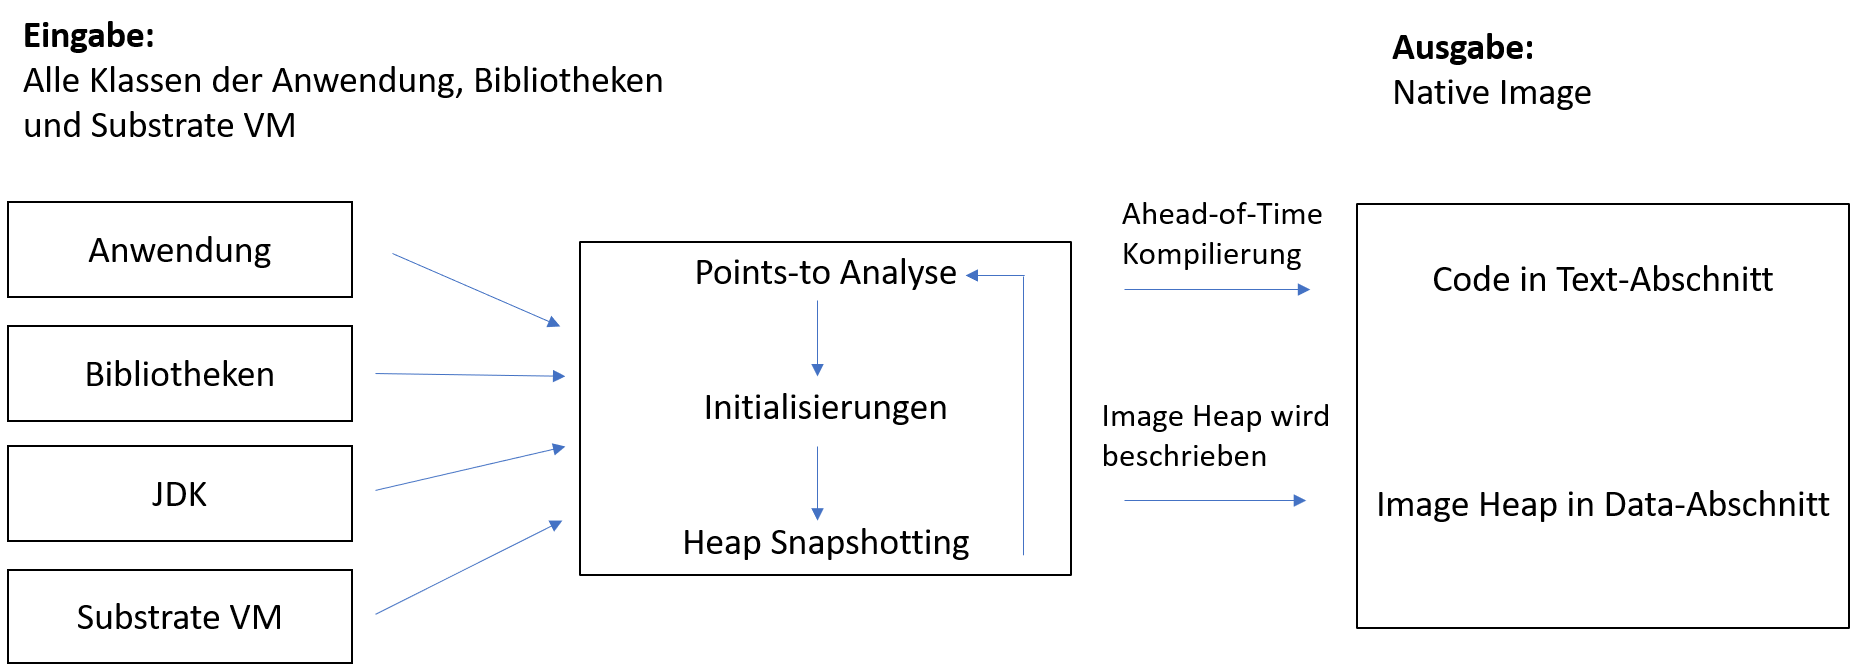
\includegraphics[width=1\textwidth]{resources/GraalVM_BuildTime.png}
	\caption{NativeImage Build-Vorgang}
	\label{fig:system_buildtime}
\end{figure}

\begin{todo}
	Bild überarbeiten, und neu einfügen.
\end{todo}

Die Points-To Analyse und das Heapsnapshotting werden iterativ durchgeführt bis ein definierter Punkt erreicht ist. Zudem werden die registrierten Callbacks der Anwendung, 
die über die Feature-API von GraalVM nutzbar sind, in diesem Zuge auch ausgeführt. Das Ergebnis dieses Prozesses ist eine Liste von, zur Laufzeit, erreichbaren Klassen, 
Methoden und Feldern, sowie ein Objekt-Graph mit erreichbaren Objekten. Im Letzten Schritt des Build-Vorgangs werden die erreichbaren Methoden zu Maschinencode kompiliert
 und der Objekt-Graph wird als \textit{image heap} ausgeschrieben, und in die Form des zur Laufzeit tatsächlich vorhandenen Heaps transformiert. Danach wird der Maschinencode 
 in die Text-Section, und der image heap in die Data-Section \parencite[Fig. 1-13]{TISC1995} des native image geschrieben. Der gesamte Prozess wird \textit{image build time} genannt\parencite{Wimmer2019}.
Die Anwendung welche die genannten Vorgänge übernimmt, ist der \textit{image builder}. Der \textit{image builder} selber ist eine Java-Anwendung. Sowohl die Pointer-Analyse 
und das ahead-of-time-Compiling, als auch das Ausführen der Klasseninitializer und Callback-Funktionen, werden also von ein und derselben Java VM
 übernommen.\footnote{Das heißt wiederrum, dass bei der \textit{image build time}, die Objekte, aus denen sich der image heap zusammensetzt,
 normale Objekte im Java Heap des \textit{image builder} sind.}

\newpage
\subsection{Points-to Analyse}
\label{subsec:pointsto}

Die Points-To Analysis (dt. Pointer-Analyse) ist eine Technik zur Berechnung der Menge von Objekten bzw. dessen Speicherbereichen, auf die eine Programm Variable zur Laufzeit zeigen kann\parencite{Hind2001, Smaragdakis2015}. 
Da der komplette Quellcode des zu analysierenden Programmes vorliegen muss, ist die Pointer-Analyse eine statische Analysetechnik.

Die Pointer Analyse startet mit allen Eingangspunkten, beispielsweise der main()-Methode. Dann werden iterativ alle erreichbaren Methoden verarbeitet, bis ein Fixpunkt erreicht ist. 
Der Java-Bytecode wird durch das Frontend des Compilers\footnote{das Frontend ist eine von 3 Stufen des Kompilierungsvorganges (Front end, Middle end, Back end), auch Analysephase genannt. Dabei wird der Code analyisiert, strukturiert und auf Fehler geprüft.} in eine Zwischenform 
überführt (engl. intermediate representation = IR), die das Programm repräsentiert und weitere Optimierungen und Transformationen ermöglicht\parencite{Simon2015}. Diese Zwischenform wird als nächstes in einen 
sog. \textit{type-flow graph} konvertiert. Jeder Knoten stellt eine Operation auf einem Objekttypen dar. Die gerichteten Kanten verlaufen von der Definition des Objektes bis zur tatsächlichen Verwendung. 
Jeder Knoten verwaltet eine Liste mit Typen (engl. \textit{type state}), die diesen Knoten erreichen können (siehe Abbildung~\ref{fig:typeflowgraph}). Die Listen werden durch die Kanten des Graphen propagiert. Sobald einer Liste Typen hinzugefügt werden, wird die Änderung an alle weiteren Verwendungen (Kindelemente eines Knotens) propagiert. Typlisten dürfen nur Elemente hinzugefügt werden, und keine Elemente gelöscht werden, damit sichergestellt ist das die Analyse den Fixpunkt erreicht und terminiert. Für jeden Typ, schaut die Pointer Analyse ob  dieser instanziiert ist. Falls dem so ist, wird er 
 durch Bytecodes markiert. Für jedes Feld, wird separat ermittelt ob die Felder während der Laufzeit nur gelesen oder auch geschrieben werden\parencite{Wimmer2019}, und als \textit{write} oder {read} markiert. Felder die als \textit{read} markiert sind, werden bereits während der Ahead-of-time Kompilierung berechnet, statt erst zur Laufzeit (sog. \textit{constant-folding}, \parencite[Kapitel 4.2]{Grumberg2014}).

\begin{figure}[!ht]
%figure full paperwidth and trim the left and right empty space from it
   \makebox[\textwidth]{
     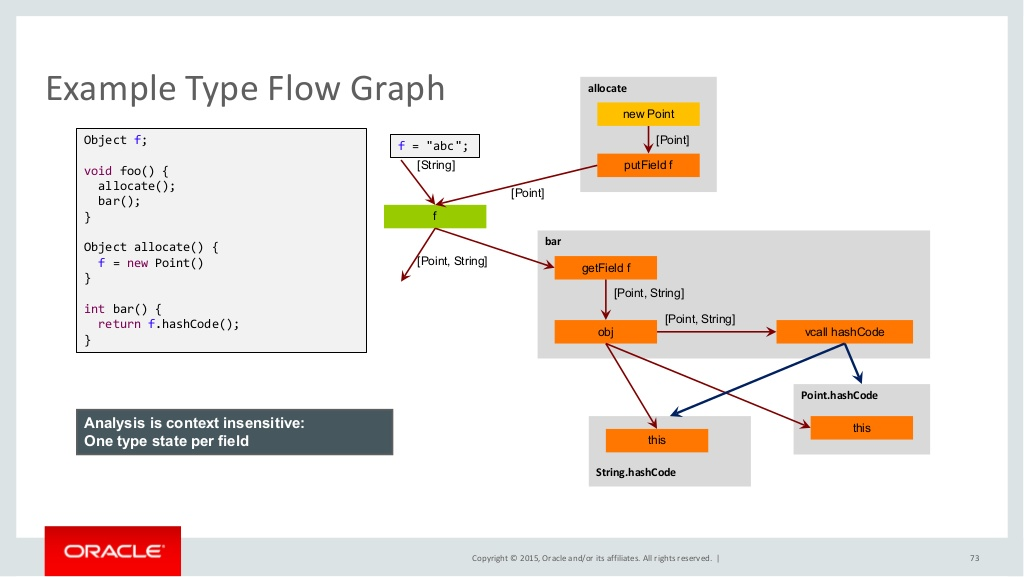
\includegraphics[trim = 8mm 0mm 16mm 0mm,width=1.1\paperwidth]{resources/graal-tutorial-at-cgo-2015.jpg}
   }
\caption{Type-flow Graph, \parencite[Folie 71 \& 72]{Wimmer2015}}
	\label{fig:typeflowgraph}
\end{figure}

\newpage
\subsection{Initialisierungscode}
\label{subsec:initializationcode}

%erwähnen, dass statische Methoden und Felder nun explizit angegeben werden müssen, um sie zur Buildtime auszuwerten

\newpage
\subsection{Heap Snapshotting}
\label{subsec:heapsnapshotting}
Beim Heap Snapshotting wird aus dem \textit{type-flow graph} der Pointer Analyse ein Objekt-Graph generiert.

Die Wurzelzeiger (eng. root pointers) des Graphen sind statische Objekt Felder, die von der Pointer Analyse als \textit{read} markiert sind. Für jedes, als \textit{read} markierte, Objekt wird nun geprüft welche weiteren Objekte durch dessen Felder erreichbar sind. 
Dafür werden die Felder nachverfolgt, indem die Feldwerte durch Reflection gelesen werden. Dies ist möglich, da der \textit{image builder} eine Java Anwendung ist.
 Falls die Klasse des Feldwertes von der Pointer-Analyse noch nicht als möglicher Typ für das Feld ermittelt 
 wurde, wird die Klasse als weiterer Feldtyp des Feldes im \textit{type-flow graph} registriert (siehe Abbildung~\ref{fig:typeflowgraph}).

Nach dem Heap Snapshotting wird die Pointer-Analyse wieder ausgeführt, um den neuen Typ des Feldes allen transitiven Verwendungen des Feldes zu propagieren. Dies geschieht durch den \textit{type-flow graph}. 
Da im \textit{type-flow graph} neue Typen hinzugekommen sind, werden auch bei der ernuten Ausführung der Klasseninitialisierer neue Initialisierer ausgeführt. Anschließend wird wieder das Heap Snapshotting ausgeführt. 
Die iterative Ausführung dieser Phasen wird beendet, sobald die Pointer-Analyse in zwei aufeinanderfolgenden Iterationen keine Änderungen findet, wenn also sowohl die Klasseninitialisierer, als auch das Heap-Snapshotting keinen neuen Code erreichbar gemacht haben.
Die Objekte des Graphen werden serializiert und in die Data-Sektion des \textit{native image} geschrieben, und bilden somit den \textit{image heap}\parencite{Wimmer2019}.

\subsection{Ahead-of-Time Compilation}
\label{subsec:aotc}

Alle Methoden die von der Points-To Analyse als \textit{erreichbar} markiert sind, werden vom GraalVM Kompiler \textit{Ahead-of-Time(AOT)}
kompiliert und in der Text-Section des \textit{native image} platziert. Der Compiler führt alle standardmäßigen Optimierungen, wie u.A Inline-Ersetzung, Loop-Unrolling und Constant-Folding, aus.
Zudem nutzt der Compiler die Resultate der Points-To analyse um die Code-Qualität zu verbessern. Dabei werden unter Anderem alle Felder, die nicht als \textit{write} markiert sind direkt als Konstante ausgewertet und Null-Prüfungen werden entfernt, falls der Typ als \textit{niemals null}  markiert wurde.
Code der nur zur \textit{build time} aber nicht zur \textit{compile time} ausgeführt wird, wie Klasseninitialisierer, wird nicht kompiliert.


\newpage
\subsection{Isolate}
\label{subsec:isolate}

Isolates stellen mehrere voneinander unabhängige VM-Instanzen im gleichen Prozess bereit. Statt einen großen Java-Heap zu haben,
kann der Heap dadurch in mehrere kleine Teile aufgeteilt werden. Beim Erstellen eines Isolates wird ein neuer separater 
Heap angelegt, welcher den \textit{image heap} als Startpunkt referenziert. Dadurch sind alle, während des \textit{image building}
ausgeführten Initialisierungen sofort in jedem Isolat verfügbar. 
\subsection{Image Heap}
\label{subsec:imageheap}

Die Ausführung des \textit{native image} erfolgt mit einem bereits, durch das Heap-Snapshotting zur Build-Time, gefüllten Java Heap,
dem \textit{image heap}. Das Starten des executables und das Instanziieren von Isolaten in einem existierenden Prozess muss
schnell sein und wenig Speicheraufwand benötigen, damit für kurzfristige Aufgaben sofort mehrere VM-Instanzen gestartet werden können.
Um das zu gewährleisten, wird der image heap nicht für jede Instanz neu kopiert werden, sondern stattdessen auf verschiedene Speicheradressen im selben Adressraum
abgebildet. Daher sind alle Referenzen relativ zum Start des \textit{image heaps}, sowohl von bereits im image heap vorhandenen Objekten, als auch von Objekten die 
erst zur Laufzeit allokiert werden. Dadurch kann der \textit{image heap} mehrere Male im Speicher des Adressraumes abgebildet werden, und erlaubt somit
schnelles Erstellen von Isolaten, da das Replizieren des \textit{image heaps} kein Kopieren erfordert.\newline
Zudem wird der Speicheraufwand durch das, auf den
image heap angewandte, Copy-On-Write Verfahren deutlich reduziert. Dabei erhalten alle Prozesse die auf die gleiche Speicherseite zugreifen, eine flache Kopie davon, also nur Zeiger die auf die tatsächliche Speicheradressen zeigen. Solange die Prozesse die Daten lediglich auslesen, ist es nicht nötig die Daten zu kopieren oder erneut im Hauptspeicher anzulegen. Alle Prozesse greifen auf das \grqq{}Original\grqq{} zu. Erst wenn ein Prozess Daten ändert (write), wird ein neuer Datenblock angelegt(copy) und die entsprechenden Referenzen angepasst \parencite{bovet2002understanding}.
Der \textit{image heap} wird vom \textit{garbage collector} als Wurzelzeiger (root pointer) behandelt, und wird daher nicht deallokiert.

\newpage
% !TEX root = main.tex
\section{Performance Benchmarks}
\label{sec:performancebenchmarks}
//frameworks erwähnen und vergleich zu hotspot erklären
\begin{figure}[h]
	\centering
	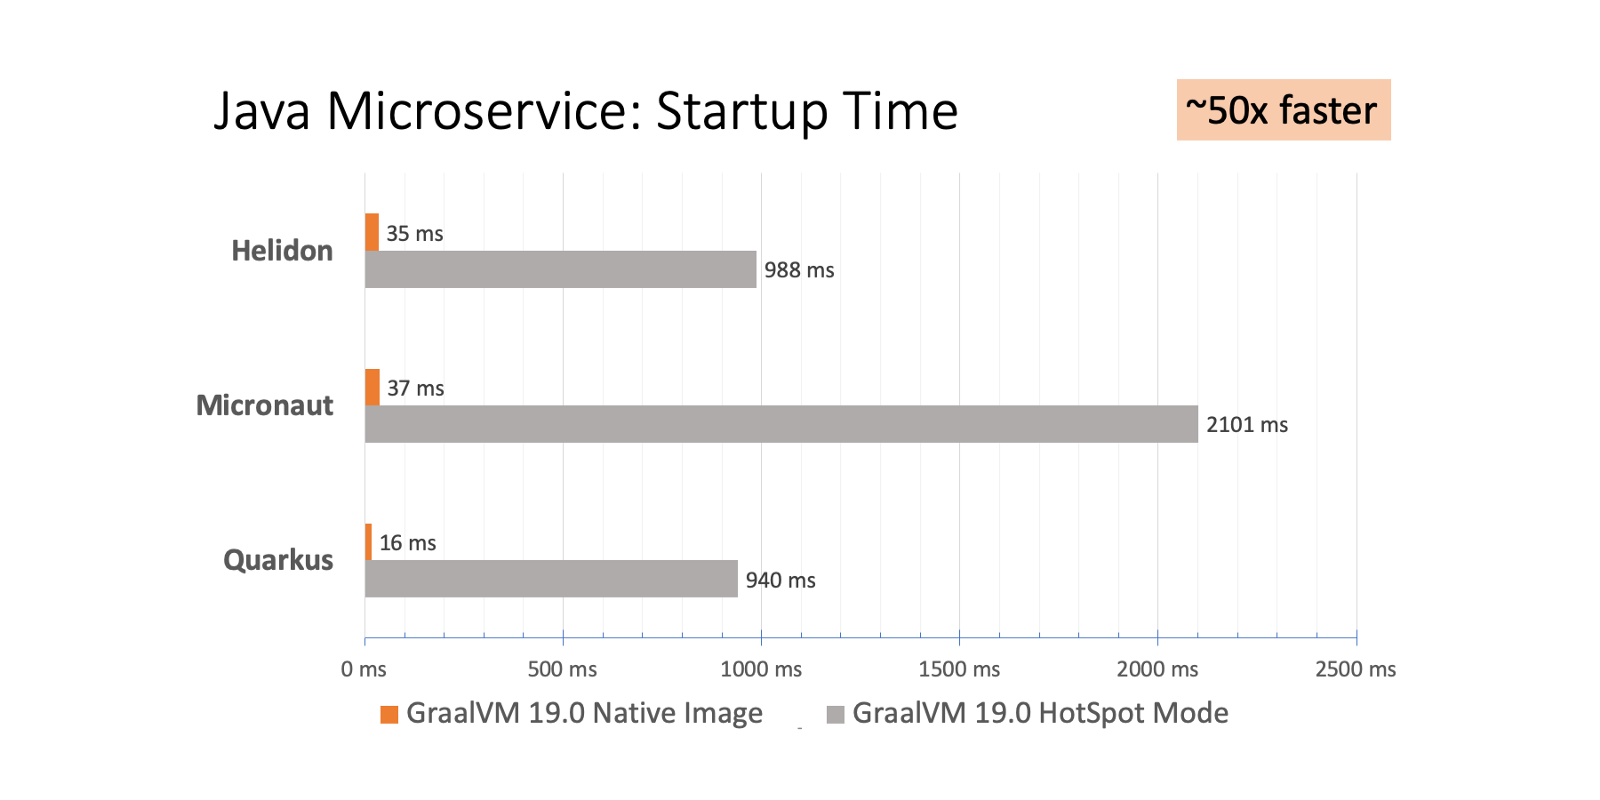
\includegraphics[width=1\textwidth]{resources/ms_startup_time.png}
	\caption{Microservices Frameworks Native Image Startzeit \cite{GraalVMBenchmarks}}
	\label{fig:system_startuptime}
\end{figure}

\begin{figure}[h]
	\centering
	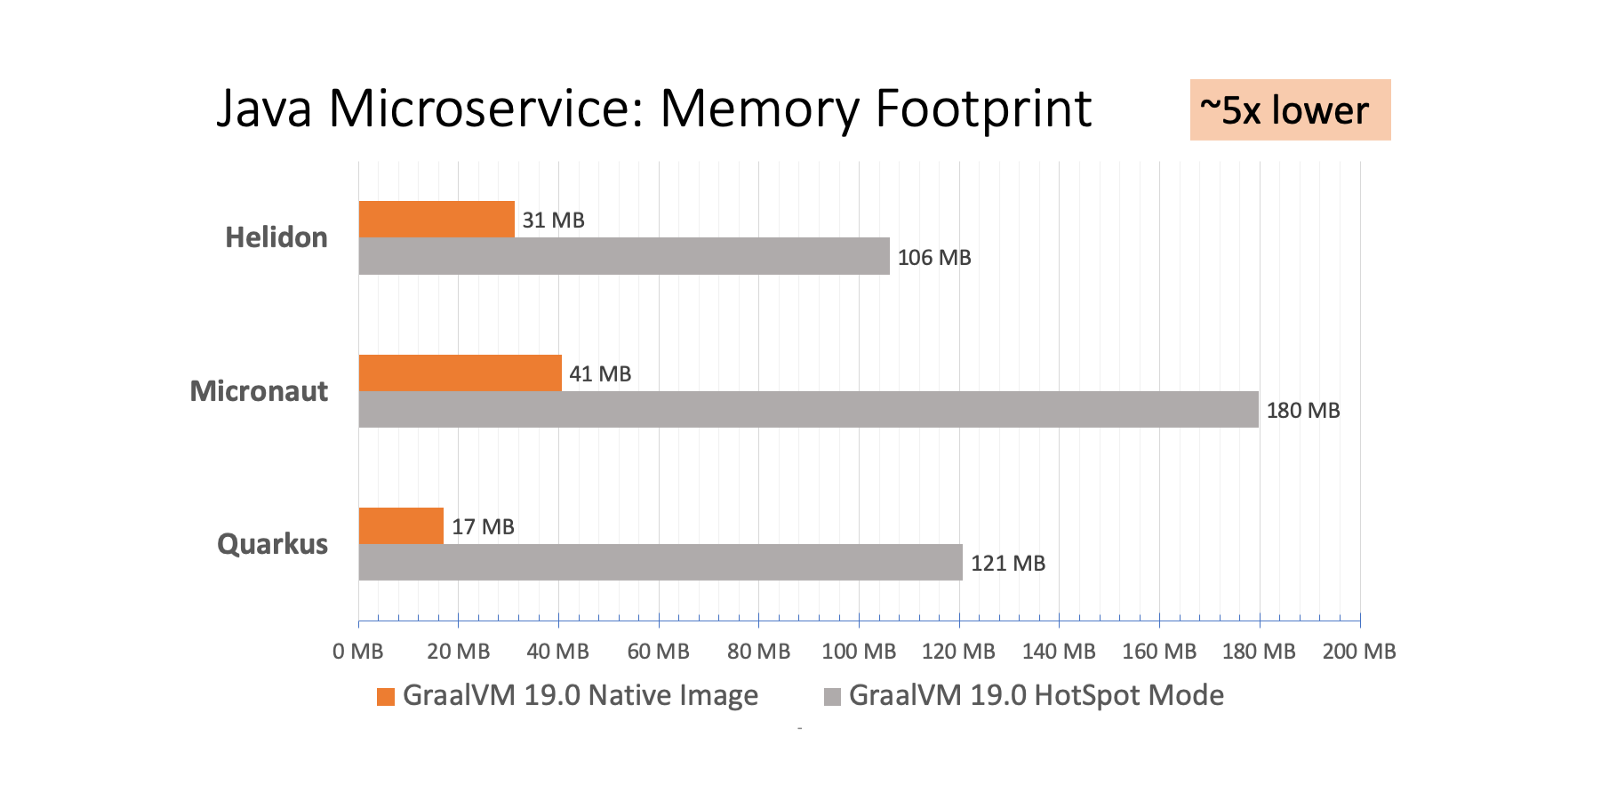
\includegraphics[width=1\textwidth]{resources/ms_memory_footprint.png}
	\caption{Microservices Frameworks Native Image Speicherbedarf \cite{GraalVMBenchmarks}}
	\label{fig:system_memory_footprint}
\end{figure}
\newpage
% !TEX root = main.tex
\section{Limitierungen}
\label{sec:limitierungen}

Die wesentliche Limitierung von \textit{native image} ist die \textit{Closed-World}-Annahme. Das bedeutet, dass der gesamte Anwendungscode zur \textit{image build time} zur Verfügung
stehen muss. Java-Features die Nutzen von dynamischer Selbstbeobachtung (engl. dynamic introspection) machen (Reflection \& Dynamic Proxy) werden durch Konfigurationsdateien unterstützt.
Im Falle von Reflection werden in der Datei die individuellen Klassen, Methoden  und Felder angegeben die durch Reflection zugänglich sind. Bei Dynamic Proxy wird die Liste der Interfaces
angegeben die dynamische Proxies definieren. Durch die Nutzung von Konfigurationsdateien werden die dynamischen Inhalte bereits zur \textit{image build time}, also ahead-of-time, bekannt und
können aufgelöst werden. Um dem Entwickler Arbeit abzunehmen werden während des Buildvorganges automatisch statische Codeanalysen durchgeführt und die Konfigurationsdateien erstellt.

Features wie Dynamic Class Loading und InvokeDynamic, die zur Laufzeit dynamisch neuen Bytecode generieren oder Methodenaufrufe einfügen und ändern können, werden nicht unterstützt.
Auch der Security Manager wird nicht unterstützt, da es kein dynamisches Klassenloading gibt und dementsprechend nur vertrauenswürdiger Code ausgeführt wird \parencite{GraalLimitiations}.
Für eine vollständige Auflistung der Features und deren Unterstützung siehe Abbildung \ref{fig:system_limitations}.
\newpage
\begin{figure}[h]
	\centering
	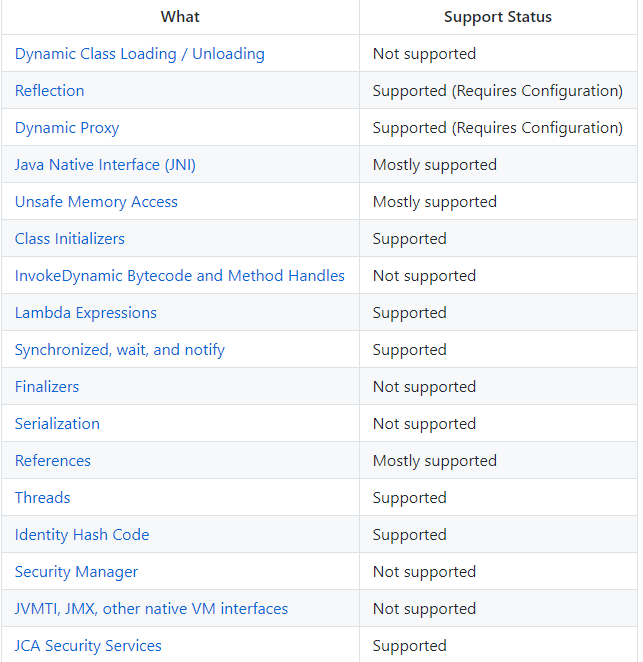
\includegraphics[width=1\textwidth]{resources/limitations.png}
	\caption{NativeImage Limitierungen \parencite{GraalLimitiations}}
	\label{fig:system_limitations}
\end{figure}
\newpage

\newpage
% !TEX root = main.tex
\section{Fazit}
\label{sec:fazit}

Ziel dieser Arbeit war es einen groben Überblick über das NativeImage-Modul von GraalVM zu geben, und die Funktionsweise, sowie die Systemkomponenten zu erläutern. 
Durch \textit{native image} wird ein leichtgewichtige, in sich geschlossene ausführbare Datei (executable) erzeugt. Dies geschieht indem die Points-To Analyse, das Ausführen
von Initialisierungscode und Heap-Snapshotting iterativ ausgeführt werden und anschließend die ahead-of-time Kompilierung erfolgt.

Durch die Initialisierung der Anwendung zur Build-Time und das Nutzen des \textit{image heaps} wird eine schnelle Startzeit, eine geringe Speichernutzung und eine gute Spitzenleistung
ermöglicht.  Zur geringeren Speichernutzung trägt auch der Umstand bei, dass es nicht mehr notwendig ist die gesamte JVM (lediglich die SubstrateVM) während der Laufzeit laufen zu lassen,
 da keine Codeoptimierungen zur Laufzeit durch den JIT-Compiler und Profiler stattfinden. Beim Vergleich populärer Java-Microservice Frameworks konnte im Durchschnitt eine um den Faktor 5 verbesserte Speichernutzung
und um den Faktor 50 verbesserte Startzeit gemessen werden, wenn statt des GraalVM HotSpot Mode GraalVM Native Image verwendet wird.

Dadurch eignet sich die Nutzung von GraalVM Native Image für die Nutzung von Java in Microservices und Serverless Cloud Functions, da hier bei jedem Start eines Services oder einer Funktion 
Kosten entsprechend der Startzeit und der Speichernutzung verursacht werden, und somit die Startzeit und der Speicherbedarf höchste Priorität haben. 
Sobald allerdings der Heap Dimensionen von mehreren Gbyte - Tbyte annimmt und/oder Klassen bzw. andere Teile des Codes erst zur Laufzeit bekannt werden, und somit die Closed-World Annahme verletzen,
 eignet sich die Java HotSpotVM besser. 

\newpage

\section*{Literaturverzeichnis}
\renewcommand{\refname}{}
\vspace{-20pt}
\printbibliography

\newpage

\end{document}
